\documentclass{beamer}
\usepackage{latexsym} 
\usepackage{graphicx}
\usetheme{Warsaw}

\title{Chapter 3}
\subtitle{A Tour of Machine Learning Classifiers Using Scikit-learn}

\begin{document}

\maketitle

\begin{frame}
  \frametitle{Choosing a classification algorithm}
  \begin{itemize}
  \item No classifier works best across all scenarios (``no free lunch'' theorem)
  \item Always need to consider the specifics of the problem
  \item Solving a problem within supervised ML framework:
    \begin{enumerate}
    \item Select features
    \item Choose performance metrics
    \item Choose classifier and optimization algorithm
    \item Evaluate performance of the model
    \item Tune the classifier
    \end{enumerate}
  \end{itemize}
\end{frame}

\begin{frame}
  \frametitle{Perceptron implementation} \href{https://github.com/rasbt/python-machine-learning-book/blob/master/code/ch03/ch03.ipynb}{\beamergotobutton{iPython notebook on github}}
\end{frame}

\begin{frame}
  \frametitle{Modeling class probabilities}
  \begin{itemize}
  \item What happens if the classes are not linearly separable?
  \item Weights never stop updating as long as there is at least one misclassified example in each epoch
  \item Logistic regression is a better option
    \item Note that despite the name this is a classification model
  \end{itemize}
\end{frame}

\begin{frame}
  \frametitle{Logistic regression model}
  \begin{itemize}
  \item This is a ``go to'' model for classification
  \item Designed for binary classification but can be extended to multiclass
  \item Odds ratio
    \[
    \frac{p}{(1-p)}
    \]
    Where $p$ is the probability of the positive class  (class label $y=1$). E.g. the probability that a patient has a certain disease.
  \item Logit function
    \[
    logit(p) = \log \frac{p}{1-p}
    \]
  \end{itemize}
\end{frame}

\begin{frame}
  \frametitle{Modeling logit function}
  \begin{itemize}
  \item We model the logit function as a linear combination of features (dot product of feature values and weights)
    \[
    logit ( p (y=1 | \mathbf{x})) = w_0 x_0 + w_1 x_1 + \cdots + w_m x_m = \sum^{m}_{i=0} w_i x_i = \mathbf{w}^T \mathbf{x}.
    \]
    Where $p(y=1 | \mathbf{x})$ s the conditional probability that a particular sample belongs to class 1 given its features $\mathbf{x}$
  \item This is equivalent to expressing $p$ as
    \[
    p(y = 1 | \mathbf{x}) = \frac{1}{1 + e^{-\mathbf{w}^T \mathbf{x}}}
    \]
  \end{itemize}
\end{frame}

\begin{frame}
  \frametitle{Logistic Sigmoid}
  \begin{itemize}
  \item Logistic function (aka sigmoid function)
    \[
    \phi(z) = \frac{1}{1+e^{-z}}.
    \]
  \item S-shaped curve
  \end{itemize}
  \center
  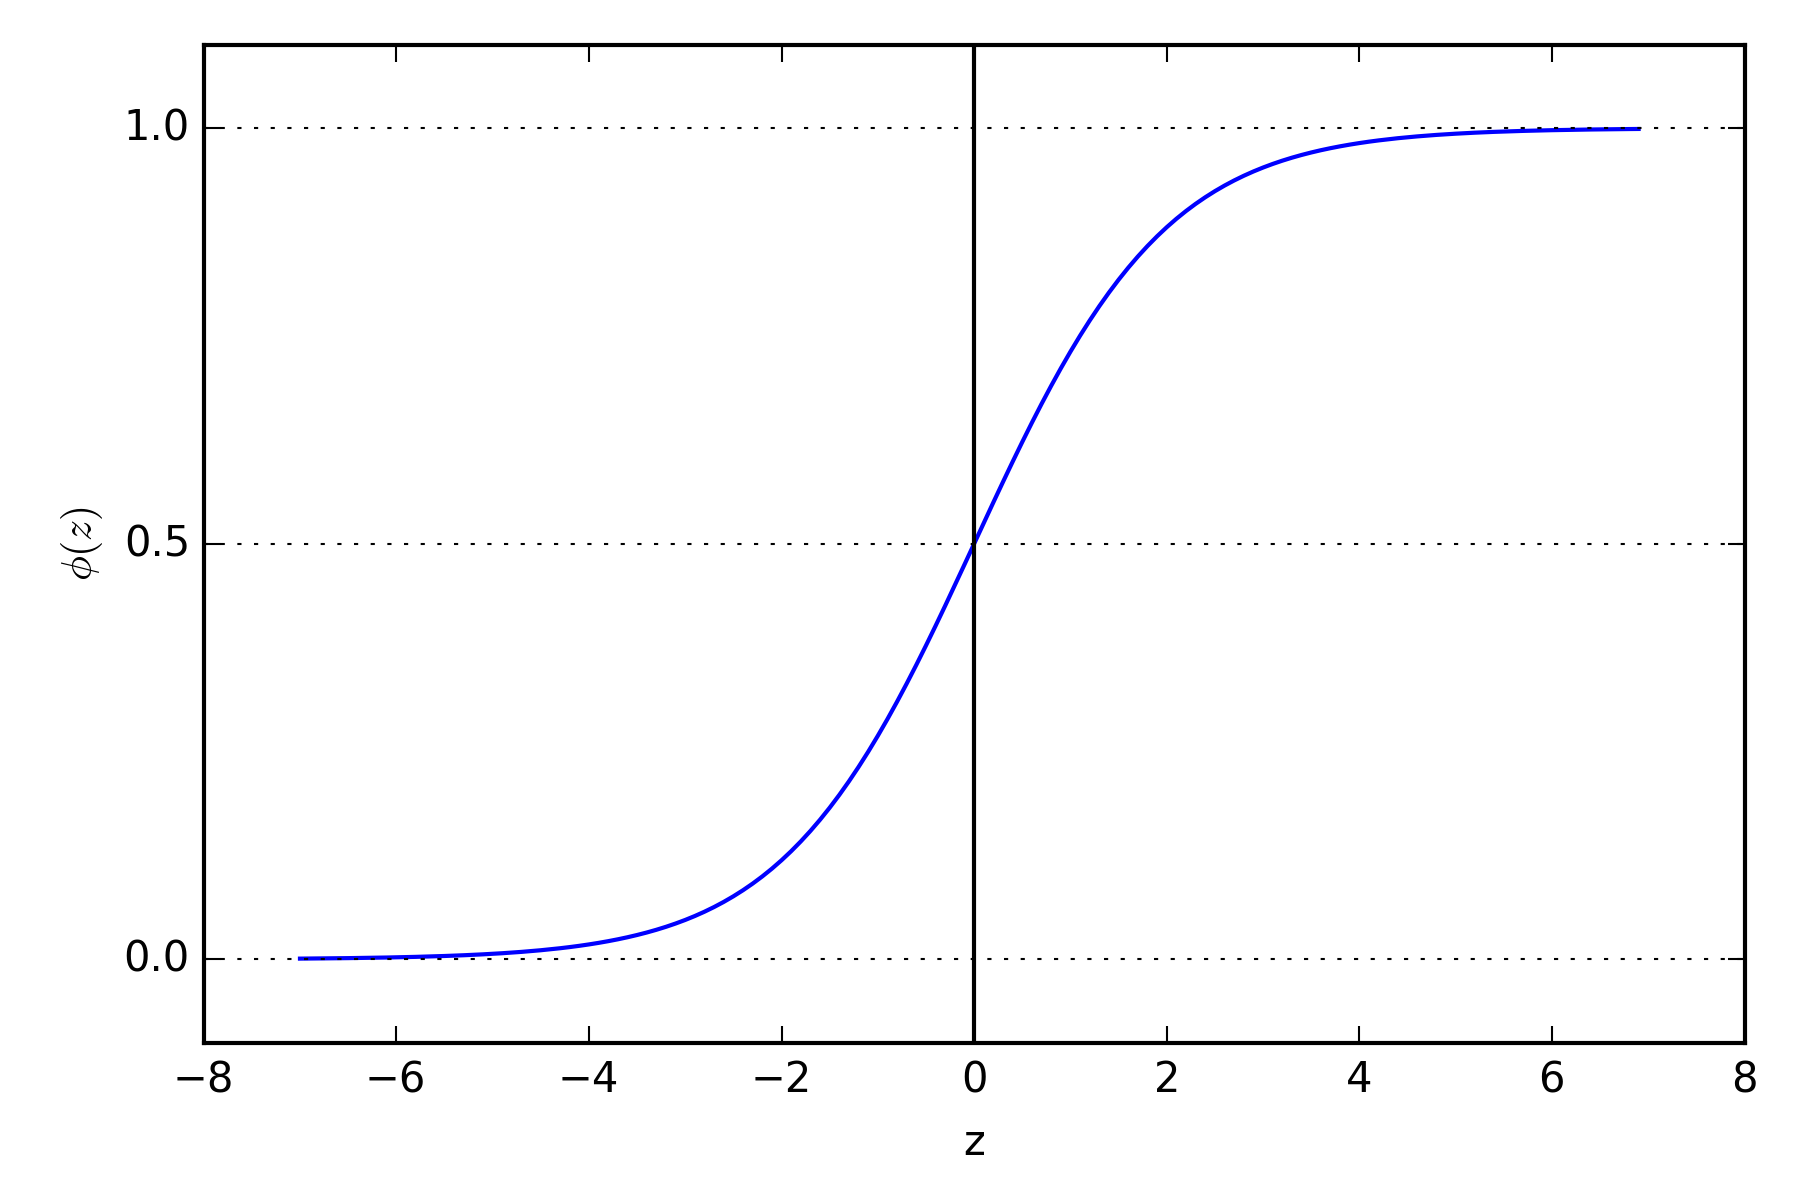
\includegraphics[scale=0.5]{Code/ch03/images/03_02.png}
\end{frame}

\begin{frame}
  \frametitle{Relationship with Adaline}
  \begin{itemize}
  \item In Adaline, we used the identify function as the activation function
  \item In logistic regression, we use instead use the sigmoid function
  \end{itemize}
  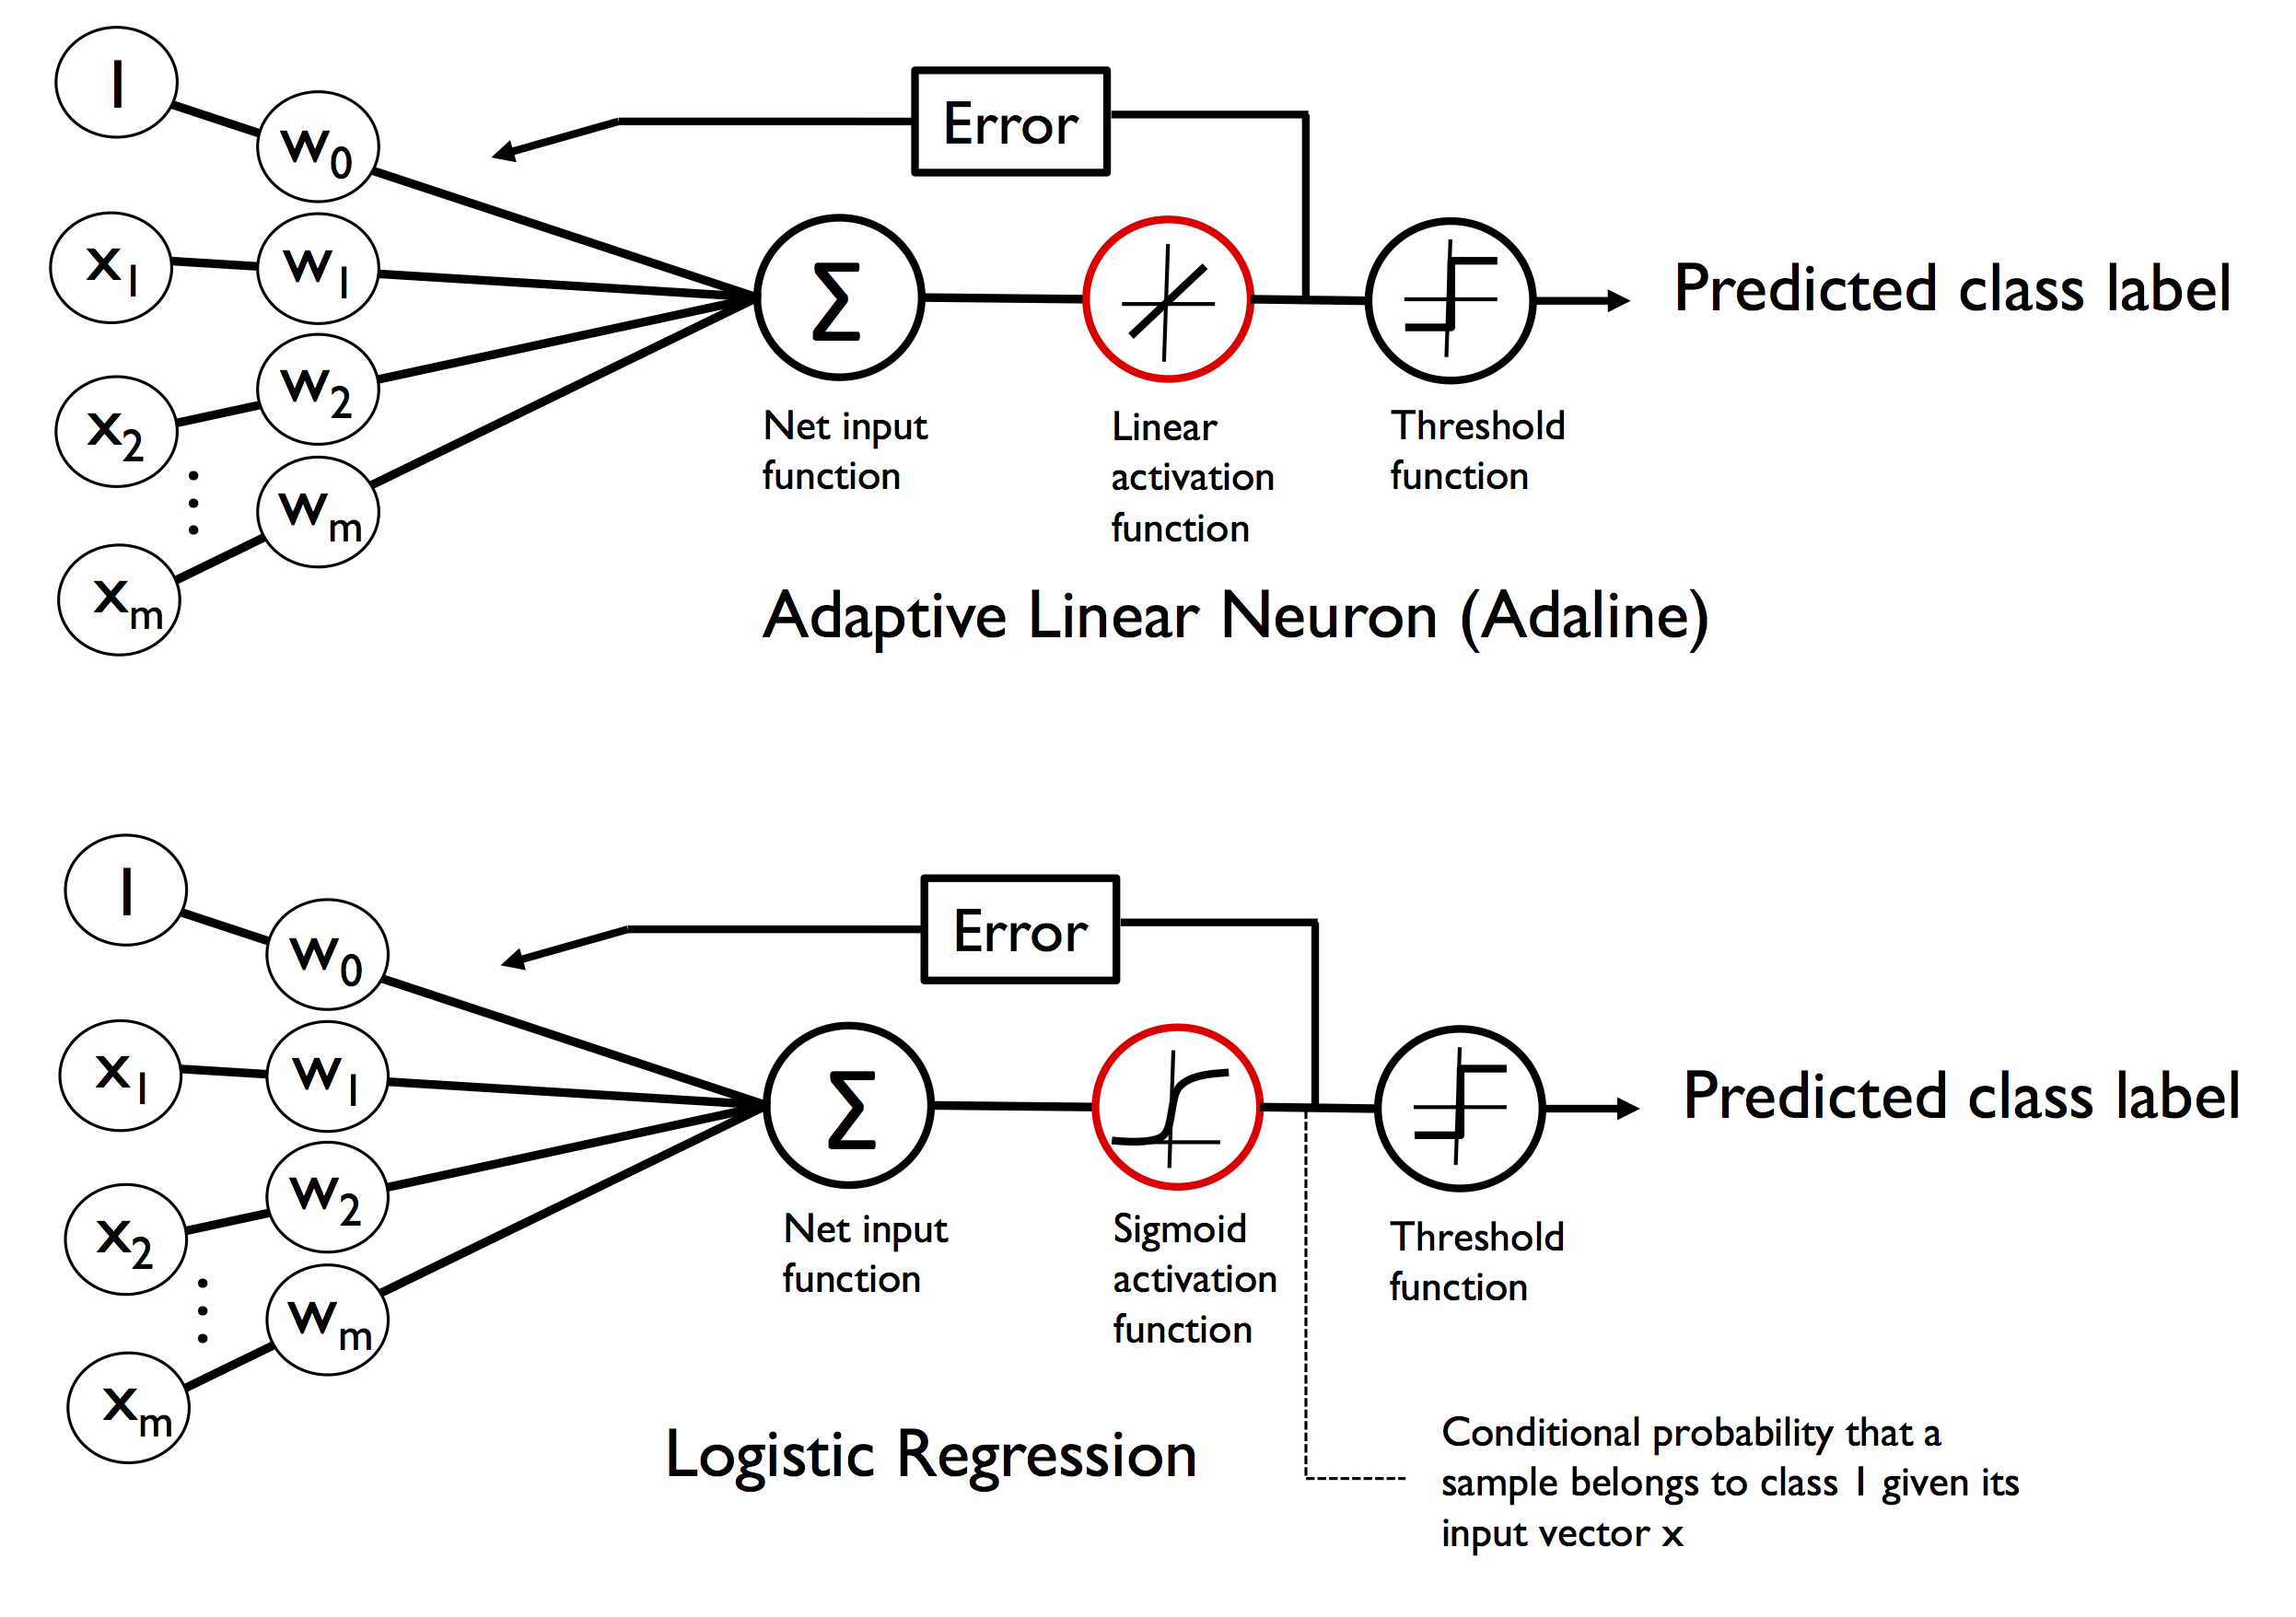
\includegraphics[width=\textwidth]{Code/ch03/images/03_03.png}
\end{frame}

\begin{frame}
  \frametitle{Probability distribution over classes}
  \begin{itemize}
  \item Output of the sigmoid often interpreted as probability
  \item E.g. $P(y=1 | \mathbf{x};\mathbf{w}) = 0.8$
  \item Probability can be converted to a binary outcome (quantizer)
  \[ \hat{y}= \begin{cases} 
    1 & \text{ if } \phi(z) \ge 0.5 \\
    0 & \text{ otherwise }.
    \end{cases}
  \]
\item Which is equivalent to the following
  \[ \hat{y}= \begin{cases} 
    1 & \text{ if } \phi(z) \ge 0.0 \\
    0 & \text{ otherwise }
    \end{cases}
  \]
  \item For many applications (e.g. weather forecasting), we want the probability
  \end{itemize}
\end{frame}

\begin{frame}
  \frametitle{Learning the weights}
  \begin{itemize}
  \item Previously we minimized the sum-squared-error cost function
    \[
    J(\mathbf{w}) = \frac{1}{2} \sum_i \bigg( \phi \big( z^{(i)} \big) - y^{(i)}  \bigg)^2
    \]
  \item Now we need to derive the cost function for logistic regression
  \item Define the likelihood $L$
  \end{itemize}
  \[
  L(\mathbf{w}) = P(\mathbf{y} | \mathbf{x}; \mathbf{w}) = \prod_{i=1}^{n} P \big( y^{(i)} | x^{(i)}; \mathbf{w} \big)
  \]
  \[
  L(\mathbf{w}) = \prod_{i=1}^{n} \bigg( \phi \big(z^{(i)} \big) \bigg) ^ {y^{(i)}} \bigg( 1 - \phi \big( z^{(i)} \big) \bigg)^{1-y^{(i)}}
  \]
\end{frame}

\begin{frame}
  \frametitle{Log-likelihood function}
  \begin{itemize}
  \item Maximize the likelihood function
    \[
    L(\mathbf{w}) = P(\mathbf{y} | \mathbf{x}; \mathbf{w})
    \]
    \[
    L(\mathbf{w}) = \prod_{i=1}^{n} P \big( y^{(i)} | x^{(i)}; \mathbf{w} \big) =  \prod_{i=1}^{n} \bigg( \phi \big(z^{(i)} \big) \bigg) ^ {y^{(i)}} \bigg( 1 - \phi \big( z^{(i)} \big) \bigg)^{1-y^{(i)}}
    \]
  \item In practice easier to deal with the natural log of this equation
    \[
    l(\mathbf{w}) = \log L(\mathbf{w})
    \]
    \[
    l(\mathbf{w}) = \sum_{i=1}^{n} \Bigg[ y^{(i)} \log \bigg(\phi \big( z^{(i)} \big) \bigg) + \bigg(1 - y^{(i)} \bigg) \log \bigg( 1 - \phi \big( z^{i()} \big) \bigg)  \Bigg]
    \]
    \item Easier to take derivative + fewer numerical underflow issues
  \end{itemize}
\end{frame}

\begin{frame}
  \frametitle{Cost function}
  \begin{itemize}
  \item Rewrite likelihood as a cost function
    \[
    J(\mathbf{w}) = \sum_{i=1}^{n} \Bigg[- y^{(i)} \log \bigg(\phi \big( z^{(i)} \big) \bigg) - \bigg(1 - y^{(i)} \bigg) \log \bigg( 1 - \phi \big( z^{i()} \big) \bigg)  \Bigg]
    \]
  \item Can now be minimized using gradient descent
  \end{itemize} \href{https://github.com/rasbt/python-machine-learning-book/blob/master/code/ch03/ch03.ipynb}{\beamergotobutton{iPython notebook on github}}
\end{frame}

\begin{frame}
  \frametitle{Weight update derivation}
  Calculate the partial derivative of the log-likelihood function with respect to the $j$th weight:
  \[
  \frac{\partial}{\partial w_j} l(\mathbf{w}) = \Bigg( y \frac{1}{\phi(z)}  - (1-y) \frac{1}{1-\phi(z)}   \Bigg)   \frac{\partial}{\partial w_j} \phi(z)
  \]
  Partial derivative of the sigmoid function:
  \[
  \frac{\partial}{\partial z} \phi(z) = \frac{\partial}{\partial z} \frac{1}{1 + e^{-1}} = \frac{1}{\big( 1 + e^{-z}\big)^2} e^{-z} = \frac{1}{1 + e^{-z}} \bigg( 1 - \frac{1}{1 + e^{-z}} \bigg)
  \]
  \[
  = \phi(z)(1-\phi(z)).
  \]
\end{frame}

\begin{frame}
  \frametitle{Weight update derivation}
  Resubstitute $\frac{\partial}{\partial z} \phi(z) = \phi(z)(1-\phi(z))$ to obtain:
  \begin{equation*}
  \begin{split}
    & \Bigg( y \frac{1}{\phi(z)} - (1-y) \frac{1}{1-\phi(z)} \Bigg) \frac{\partial}{\partial w_j} \phi(z) \\
    & = \Bigg( y \frac{1}{\phi(z)} - (1-y) \frac{1}{1-\phi(z)} \Bigg) \phi(z) \big(1 - \phi(z)\big) \frac{\partial}{\partial w_j} z \\
    & = \bigg(  y \big( 1 - \phi(z)   \big) - (1-y) \phi(z)  \bigg) x_j \\
    & = \big( y - \phi(z)  \big) x_j
  \end{split}
  \end{equation*}
\end{frame}

\begin{frame}
  \frametitle{Overfitting}
  \begin{itemize}
  \item Sometimes model performs well on training data but does not generalize well to unsee data (test data)
  \item This is overfitting
  \item If a model suffers from overfitting, the model has a high variance
  \item This is often caused by a model that's too complex
  \item Underfitting can also occur (high bias)
  \item Underfitting is caused by a model's not being complex enough
  \item Both suffer from low performance on unseen data
  \end{itemize}
\end{frame}

\begin{frame}
  \frametitle{Bias-variance tradeoff}
  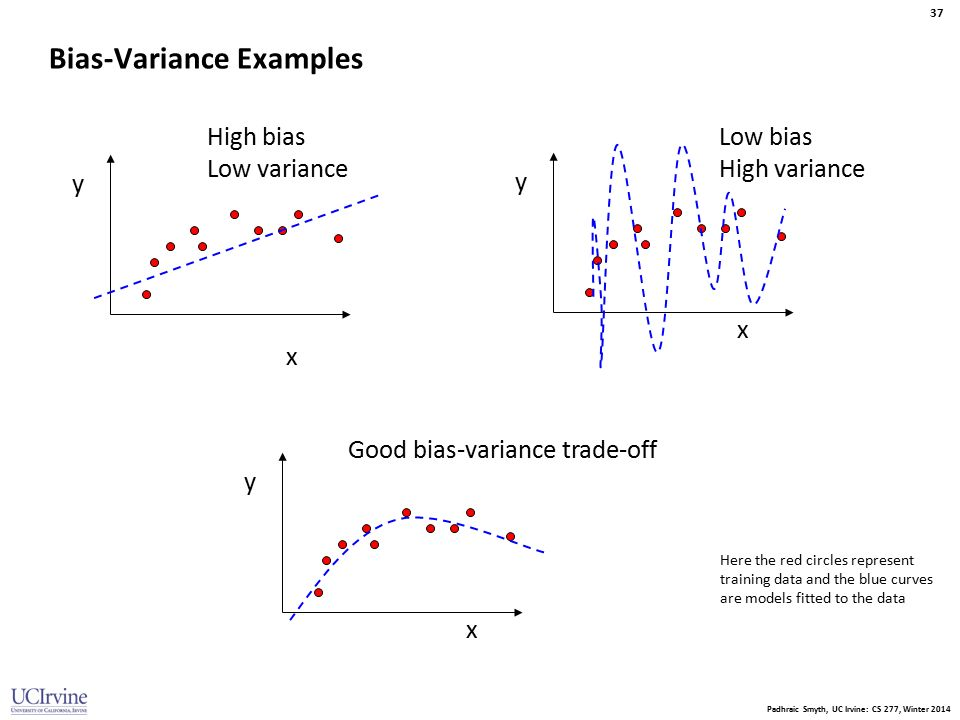
\includegraphics[scale=0.4]{Images/bias-variance.jpg}
\end{frame}

\begin{frame}
  \frametitle{Regularization}
  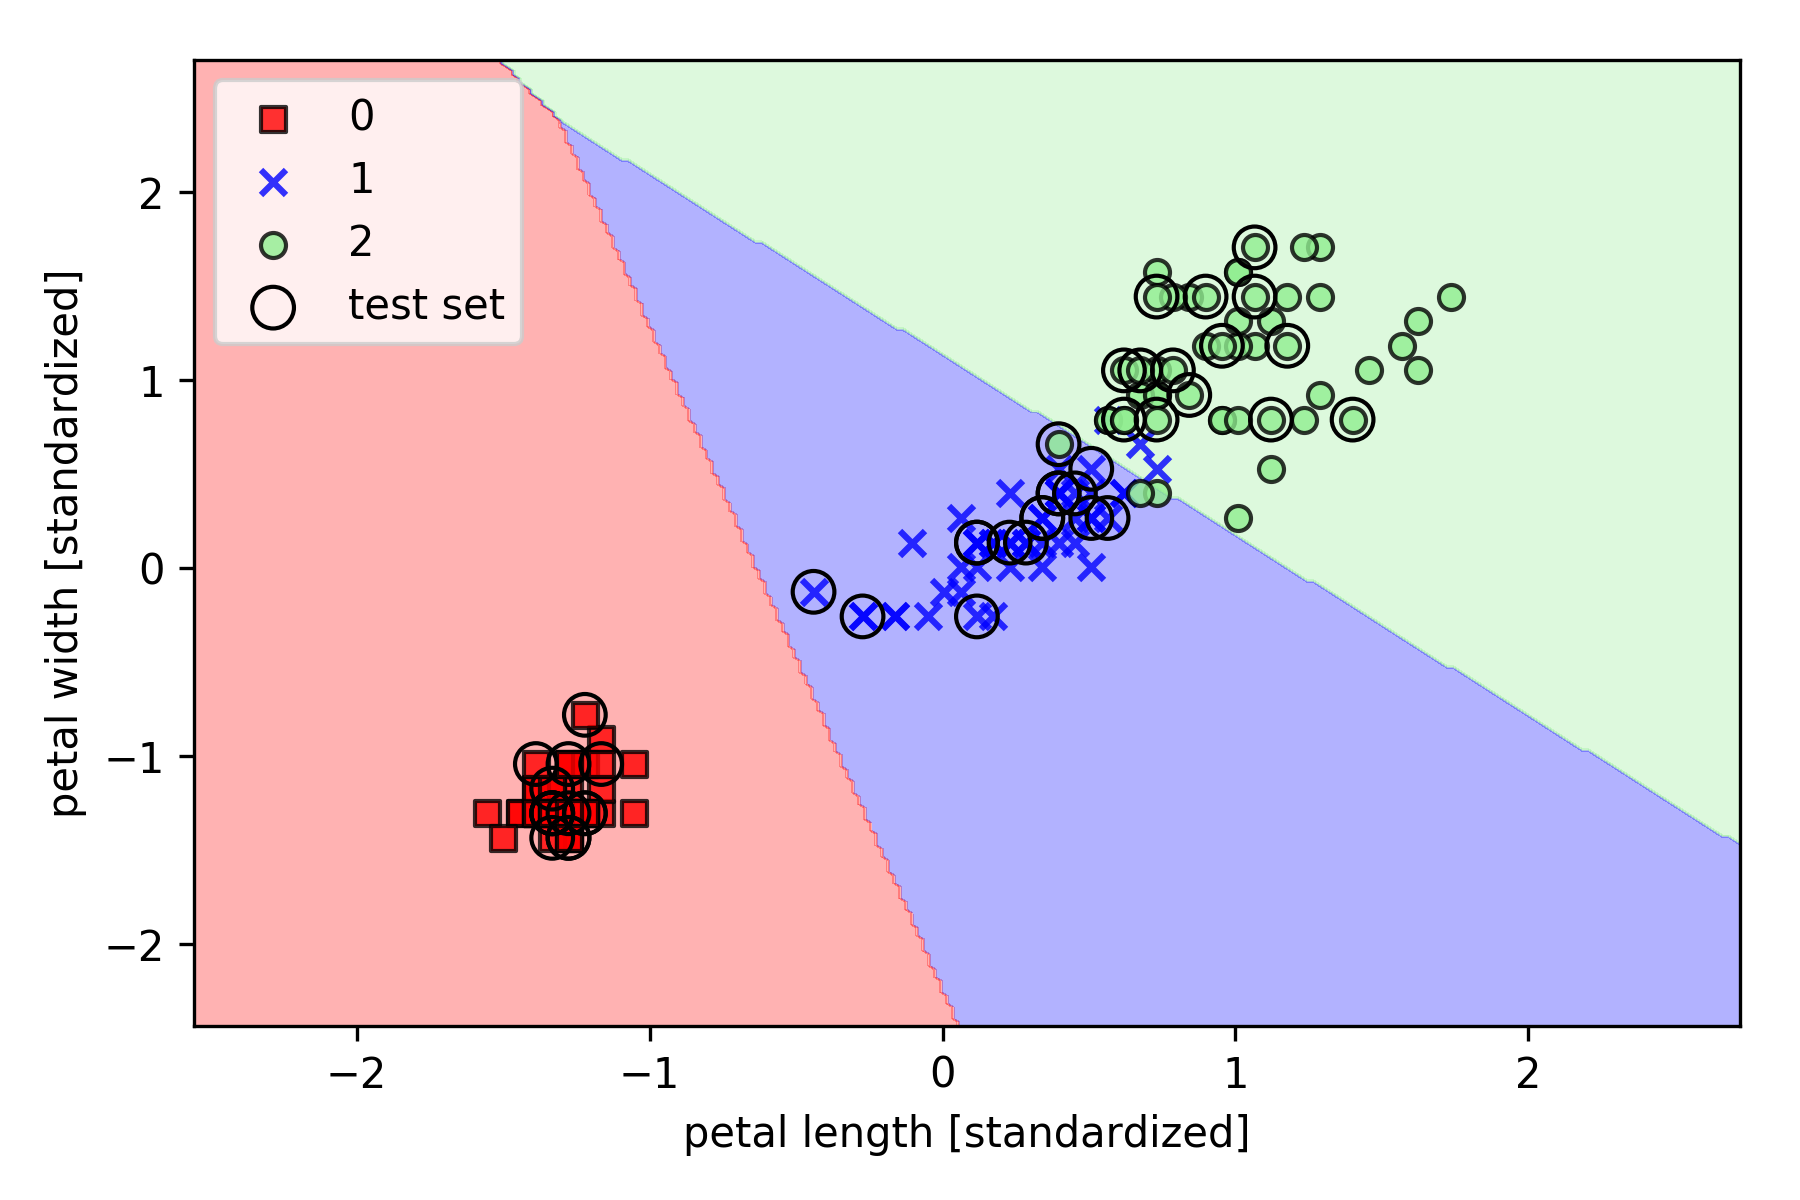
\includegraphics[scale=0.3]{Code/ch03/images/03_06.png}
  \begin{itemize}
  \item Regularization is a way to tune the complexity of the model
  \item Regularization helps to filter out noise from training data
  \item As a result, regularization prevents overfitting
  \end{itemize}
\end{frame}

\begin{frame}
  \frametitle{}
  \subsection{Tackling overfitting via regularization}
  The most common form of regularization is the so-called L2 regularization (sometimes also called L2 shrinkage or weight decay):
  \[
  \frac{\lambda}{2} \lVert \mathbf{w} \rVert^2 = \frac{\lambda}{2} \sum_{j=1}^m w_{j}^{2}
  \]
  Where $\lambda$ is the so-called regularization parameter.
  To apply regularization, we add the regularization term to the cost function, which shrinks the weights:
  \[
  J(\mathbf{w}) = \sum_{i=1}^{n} \bigg[ - y^{(i)} \log \big(  \phi(z^{(i)})  \big)  - \big( 1 - y ^{(i)} \big)  \log \big( 1 - \phi(z^{(i)})   \big)   \bigg] + \frac{\lambda}{2} \lVert \mathbf{w}\rVert^2  
  \]
\end{frame}

\begin{frame}
  \frametitle{Regularization parameter}
  \begin{itemize}
  \item We control how well we fit the training data via the regularization parameter $\lambda$
  \item By increasing $\lambda$, we increase the strength of regularization
  \item Sometimes (e.g in scikit-learn), SVM terminology is used
    \[
    C = \frac{1}{\lambda}
    \]
  \item I.e we rewrite the regularized cost function of logistic regression:
  \end{itemize}
  \[
  C \Bigg[  \sum_{i=1}^{n} \Big(   -y^{(i)} \log \big( \phi(z^{(i)} \big) - \big(  1 - y^{(i)} \big)    \Big) \log \bigg( 1 - \phi(z^{(i)}) \bigg)         \Bigg] + \frac{1}{2} \lVert \mathbf{w} \rVert^2
  \]
\end{frame}

\begin{frame}
  \frametitle{Regularization illustrated}
  \begin{itemize}
  \item Decreasing the value of $C$ means increasing the regularization strength
  \item Can be visualized by plotting L2 regularization path for two weights
  \item Display weights across multiple C values
  \item As you see, weights shrink to zero as C decreased
  \item \href{https://github.com/rasbt/python-machine-learning-book/blob/master/code/ch03/ch03.ipynb}{\beamergotobutton{iPython notebook on github}}
  \end{itemize}
\end{frame}

\begin{frame}
  \frametitle{Support Vector Machines}
  \begin{itemize}
  \item In SVMs, the optimization objective is to maximize the \textbf{margin}
  \item The margin is defined as the distance between the separating hyperlane and the training samples that are closest to this hyperplane (\textbf{support vectors})
  \item Intuitively, the larger the margin, the lower generalization error
  \item Models with small margin prone to overfitting
  \end{itemize}
\end{frame}

\begin{frame}
  \frametitle{Maximum margin classification}
  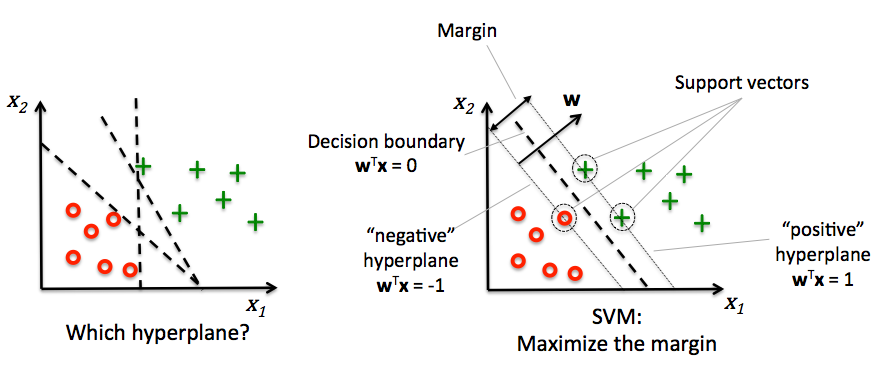
\includegraphics[width=\textwidth]{Code/ch03/images/03_07.png}
\end{frame}

\begin{frame}
  \frametitle{Mathematical intuition}
  \textit{Positive} and \textit{negative} hyperplanes that are parallel to the decision boundary, which can be expressed as follows:
  \[
  w_0 + \mathbf{w}^T \mathbf{x}_{pos} = 1
  \]
  \[
  w_0 + \mathbf{w}^T \mathbf{x}_{neg} = -1
  \]
  Distance between these two planes (prove it!), i.e. the margin:
  \[
  \frac{2}{\lVert \mathbf{w} \rVert}
  \]
  Where the length of the vector $\mathbf{w}$ is defined as follows:
  \[
  \lVert \mathbf{w} \rVert = \sqrt{\sum_{j=1}^{m} w_{j}^{2}} 
  \]
\end{frame}

\begin{frame}
  \frametitle{Constrained optimization problem}
  Minimize:
  \[
  \frac{1}{2} \lVert \mathbf{w} \rVert^2
  \]
  Subject to constraints that the samples are classified correctly:
  \[
  w_0 + \mathbf{w}^T \mathbf{x}^{(i)} \ge 1 \text{ if } y^{(i)} = 1
  \]
  \[
  w_0 + \mathbf{w}^T \mathbf{x}^{(i)}  < -1 \text{ if } y^{(i)} = -1
  \]
  These equations say that all negative and positive samples should fall respectively on one side of the negative and positive hyperplanes. This can be written more compactly:
  \[
  y^{(i)} \big(  w_0 + \mathbf{w}^T \mathbf{x}^{(i)} \big) \ge 1 \quad \forall_i
  \]
\end{frame}

\begin{frame}
  \frametitle{SVM Solution}
  Classsifier
  \[
  f(\mathbf{x}) = sgn(\mathbf{w}^T \mathbf{x} + w_0)
  \]
  Weights
  \[
  \mathbf{w} = \sum_{i=1}^N \alpha_i y_i \mathbf{x}_i
  \]
\end{frame}

\begin{frame}
  \frametitle{Slack variables / soft margin SVM}
  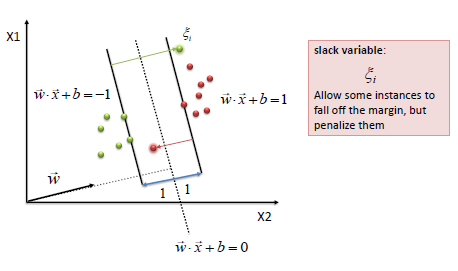
\includegraphics[width=\textwidth]{Images/svm-slack.png}
  \\
  \tiny{Source: http://www.saedsayad.com/support\_vector\_machine.htm}
\end{frame}


\begin{frame}
  \frametitle{Extending SVM to non-linearly separable cases}
  \begin{itemize}
  \item Need to relax the linear constraints
  \item To ensure convergence in presense of misclassifications
  \item Introduce slack variables $\xi$
  \end{itemize}
  \\
  \[
  \mathbf{w}^T \mathbf{x}^{(i)} \ge 1 - \xi^{(i)} \text{ if } y^{(i)} = 1
  \]
  \[
  \mathbf{w}^T \mathbf{x}^{(i)} < -1 + \xi^{(i)} \text{ if } y^{(i)} = -1
  \]
  New objective to be minimized:
  \[
  \frac{1}{2} \lVert \mathbf{w} \rVert^2 + C \Big(\sum_i \xi^{(i)} \Big)
  \]
\end{frame}

\begin{frame}
  \frametitle{Regularization in SVMs}
  \[
  \frac{1}{2} \lVert \mathbf{w} \rVert^2 + C \Big(\sum_i \xi^{(i)} \Big)
  \]
  \begin{itemize}
  \item Large values of $C$ - large error penalties
  \item Small values of $C$ - less strict about misclassifications
  \item Parameter $C$ controls width of the margin
  \item I.e. $C$ is a way to do regularization in SVMs
  \end{itemize}
\end{frame}

\begin{frame}
  \frametitle{Regularization in SVMs}
  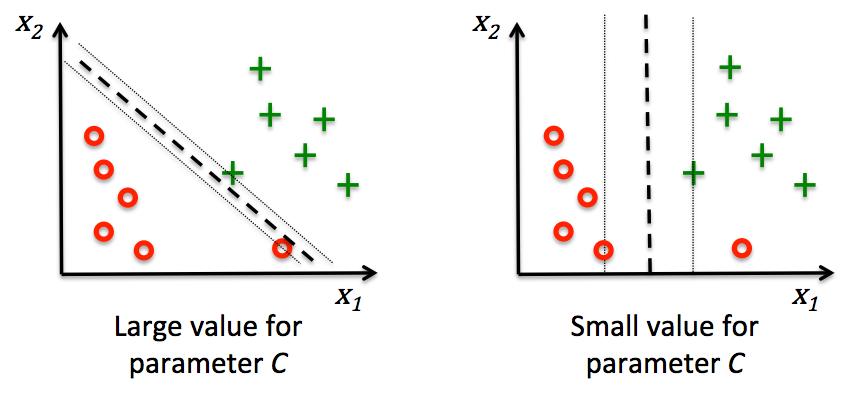
\includegraphics[width=\textwidth]{Code/ch03/images/03_08.png}
\end{frame}

\begin{frame}
  \frametitle{Exclusive OR (XOR) linear separability}
  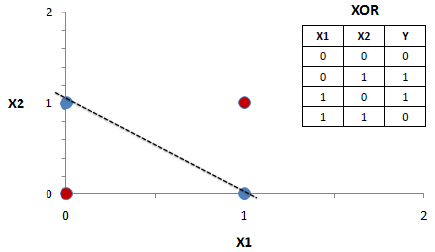
\includegraphics[width=\textwidth]{Images/xor.png}
  \\
  \tiny{Source: http://www.saedsayad.com/artificial\_neural\_network\_bkp.htm}
\end{frame}

\begin{frame}
  \frametitle{Generated XOR data}
  \begin{itemize}
  \item \href{https://github.com/rasbt/python-machine-learning-book/blob/master/code/ch03/ch03.ipynb}{\beamergotobutton{iPython notebook on github}}
  \item Kernel methods create non-linear combinations of the original features
  \item Project onto a higher dimensional space where they are separable
  \item Mapping function $\phi(\cdot)$
  \end{itemize}
  \[
  \phi(x_1, x_2) = (z_1, z_2, z_3) = (x_1, x_2, x_{1}^{2} + x_{2}^{2})
  \]
\end{frame}

\begin{frame}
  \frametitle{Turn non-separable classess are separable}
  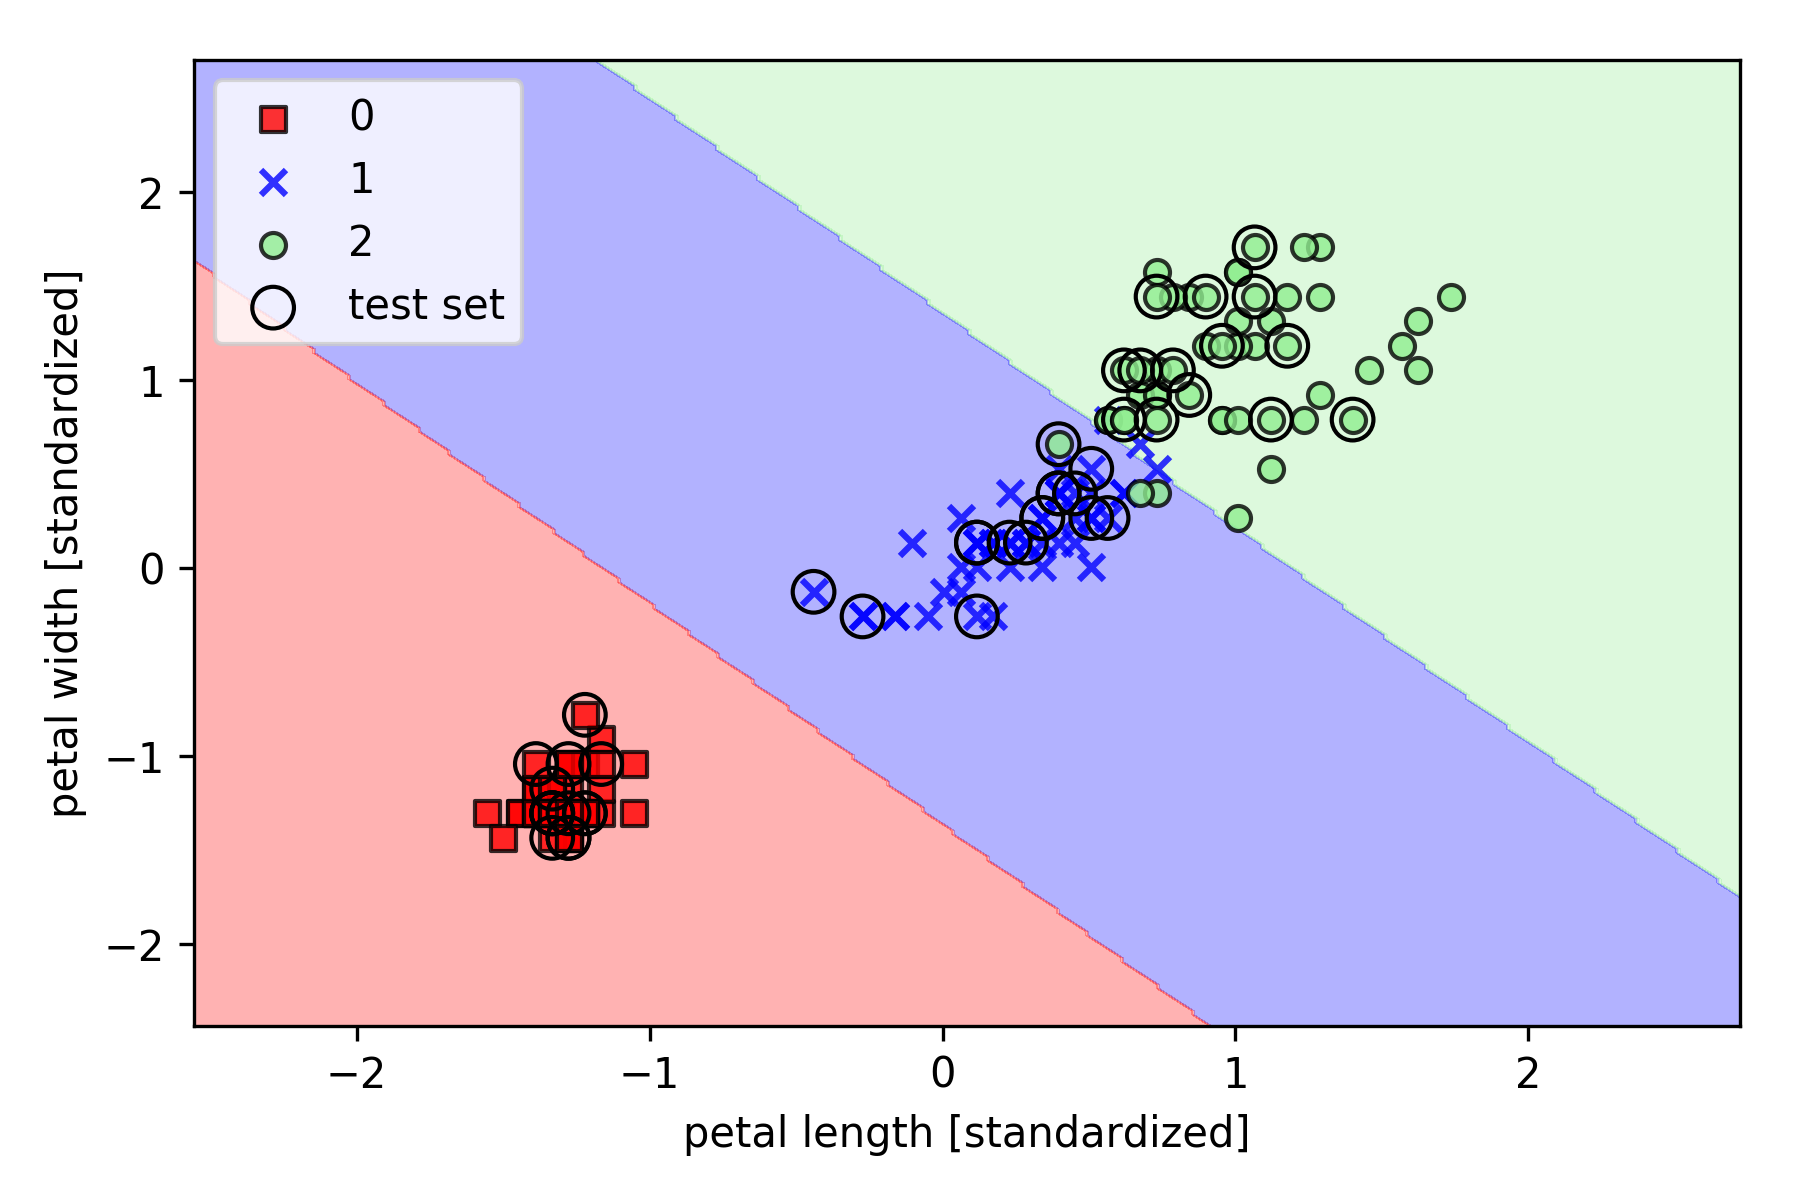
\includegraphics[width=\textwidth]{Code/ch03/images/03_11.png}
\end{frame}

\begin{frame}
  \frametitle{Kernel trick}
  General blueprint:
  \begin{itemize}
  \item Transform training data into a higher dimensional space via a mapping function $\phi(\cdot)$
  \item Train a linear SVM to classify the data in the new feature space
  \item Use the same mapping function $\phi(\cdot)$ to transform new (unseen) data
  \item Classify unseen data using the linear SVM model
  \end{itemize}
\end{frame}

\begin{frame}
  \frametitle{Problem with explicit mapping}
  \begin{itemize}
  \item The construction of the new features is computationally expensive
  \item Fortunately, we have the \textit{kernel trick}
  \item Decision boundary rely on dot products in input space
  \item Need to replace the dot product
    \[
    \mathbf{x}^{(i) \; T} \mathbf{x}^{(j)} \text{ by } \phi \big( \mathbf{x}^{(i)} \big)^T \phi \big( \mathbf{x}^{(j)} \big)
    \]
  \item No need to calculate this dot product explicitly
  \item Instead, we define a kernel function:
    \[
    k \big( \mathbf{x}^{(i)}, \mathbf{x}^{(j)}  \big) = \phi \big( \mathbf{x}^{(i)} \big)^T \phi \big( \mathbf{x}^{(j)} \big)
    \]
  \end{itemize}
\end{frame}

\begin{frame}
  \frametitle{Kernel Trick: Example}
  $\mathbf{x} = (x_1, x_2), $
  $\mathbf{z} = (z_1, z_2), $ 
  $K(\mathbf{x}, \mathbf{z}) = \langle \mathbf{x} \cdot \mathbf{z} \rangle^2$
  \[
  K(x, z) = (x_1z_1 + x_2z_2)^2 = (x_1^2z_1^2 + 2x_1z_1x_2z_2 + x_2^2z_2^2) = \\
  = \langle (x_1^2, \sqrt{2}x_1x_2, x_2^2) \cdot (z_1^2, \sqrt{2}z_1z_2, z_2^2) \rangle
  = \lange \phi(\mathbf{x}) \phi(\mathbf{z}) \rangle
  \]
  % source: http://www.cogsys.wiai.uni-bamberg.de/teaching/ss06/hs_svm/slides/SVM_and_Kernels.pdf
\end{frame}

\begin{frame}
  \frametitle{RBF Kernel}
  One of the most widely used kernels is the \textit{Radial Basis Function kernel} (RBF kernel) or Gaussian kernel:
  \[
  k \big( \mathbf{x}^{(i)}, \mathbf{x}^{(j)}  \big) = \exp \Bigg( - \frac{ \lVert \mathbf{x}^{(i)} - \mathbf{x}^{(j)} \rVert^2  }{2 \sigma^2} \Bigg)
  \]
  This is often simplified to:
  \[
  k \big( \mathbf{x}^{(i)}, \mathbf{x}^{(j)}  \big) = \exp \bigg(  -\gamma\ \lVert \mathbf{x}^{(i)} - \mathbf{x}^{(j)} \rVert^2  \bigg)
  \]
  Here, $\gamma = \frac{1}{2 \sigma^2}$ is a free parameter that is to be optimized.
\end{frame}

\begin{frame}
  \frametitle{}
  \begin{itemize}
  \item The term \textit{kernel} can be interpreted as a \textit{similarity function} between a pair of samples
  \item The minus sign inverts the distance measure into a similarity score (from 0/dissimilar to 1/very similar)
  \item Use RBF kernel to separate XOR data
  \item Vary the $\gamma$ parameter
  \item \href{https://github.com/rasbt/python-machine-learning-book/blob/master/code/ch03/ch03.ipynb}{\beamergotobutton{iPython notebook on github}}
  \end{itemize}
\end{frame}

\begin{frame}
  \frametitle{K-nearest neighbors}
  \begin{itemize}
  \item KNN is an example of a non-parametric model
  \item Parametric models learn parameters from training data
  \item Once training done, the training set not required
  \item KNN is an instance-based learner
  \end{itemize}
\end{frame}

\begin{frame}
  \frametitle{Basic KNN algorithm}
  \begin{itemize}
  \item Choose $k$ and a distance metric
  \item Find $k$ nearest neighbors of the sample to be classified
  \item Assign the class label by majority vote
  \end{itemize}
\end{frame}

\begin{frame}
  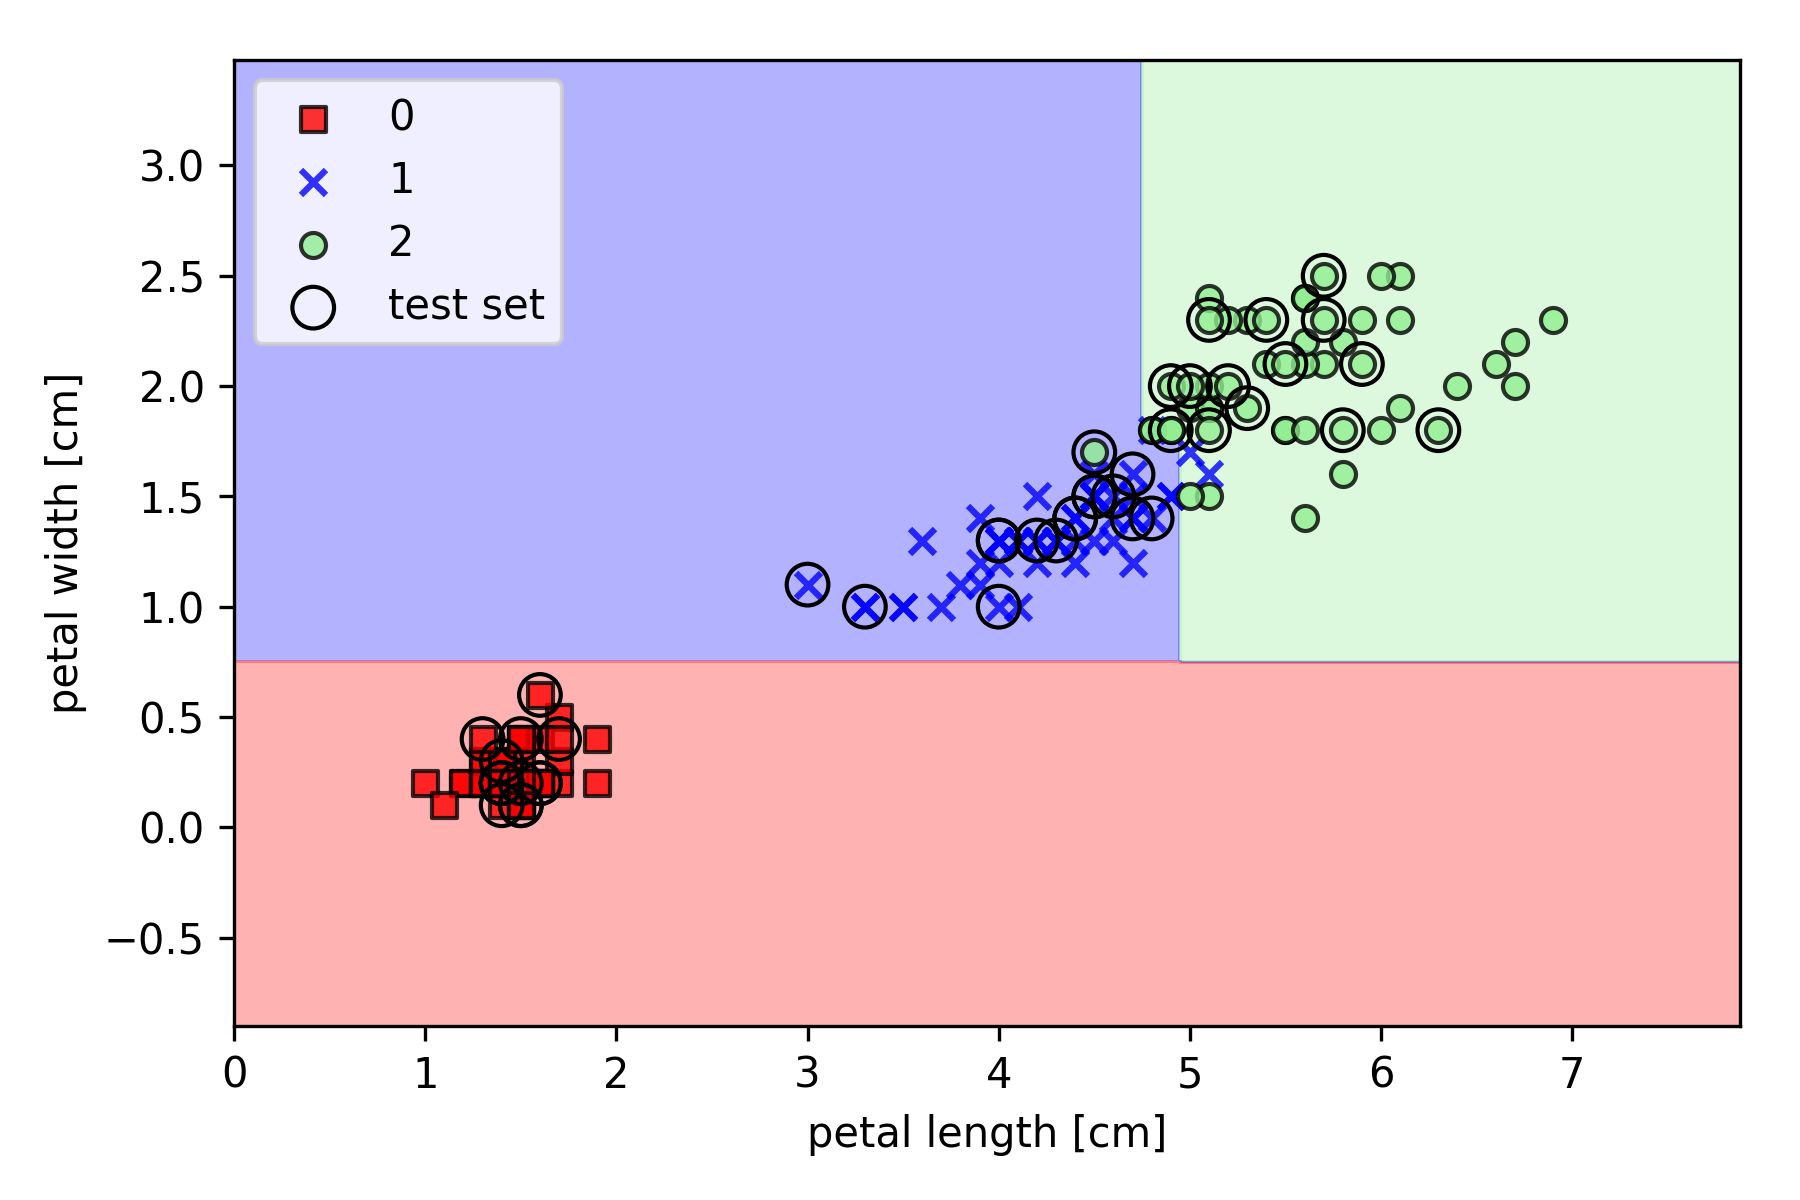
\includegraphics[height=\textheight, width=\textwidth]{Code/ch03/images/03_20.png}
\end{frame}

\begin{frame}
  \frametitle{KNN advantages}
  \begin{itemize}
  \item Classifier immediately adapts as we receive new training examples
  \item But computational complexity grows linearly with the number of samples
  \item Need efficient data structures such as KD-trees
  \end{itemize}
  Distance metrics:
  \[
  d \big(\mathbf{x}^{(i)}, \mathbf{x}^{(j)}\big) =  \sqrt[p]{\sum_k \big| x_{k}^{(i)} - x_{k}^{(j)} \big|^p } 
  \]
  Euclidean distance if we set the parameter $p=2$ \\
  Manhattan distance if we set the parameter $p=1$
\end{frame}

\end{document}
